\documentclass[tikz,border=5pt]{standalone}
\usepackage{pgfplots}
\pgfplotsset{compat=1.18}

\definecolor{corba}{HTML}{365FB3}
\definecolor{punt}{HTML}{B91C1C}

\begin{document}
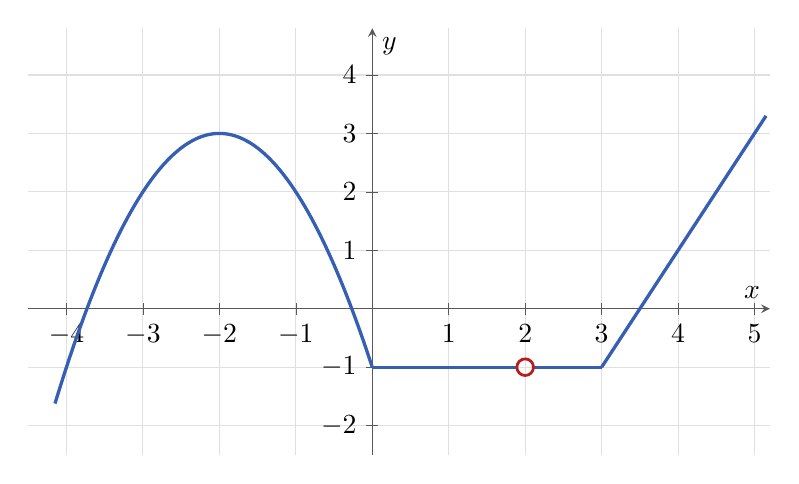
\begin{tikzpicture}
  \begin{axis}[
    width=11cm,
    height=7cm,
    axis lines=middle,
    xmin=-4.5,
    xmax=5.2,
    ymin=-2.5,
    ymax=4.8,
    xlabel={$x$},
    ylabel={$y$},
    xtick={-4,-3,-2,-1,0,1,2,3,4,5},
    ytick={-2,-1,0,1,2,3,4},
    grid=major,
    grid style={black!12},
    axis line style={black!65},
    tick style={black!65},
    clip=true,
  ]
    % Arc de paràbola amb tangent horitzontal en x=-2.
    \addplot[corba, very thick, domain=-4.15:0, samples=150]
      {-(x+2)^2+3};

    % Tram constant amb una discontinuïtat evitable en x=2.
    \addplot[corba, very thick, domain=0:1.90, samples=25] {-1};
    \addplot[corba, very thick, domain=2.10:3, samples=20] {-1};
    \addplot[
      only marks,
      mark=o,
      mark size=3pt,
      mark options={draw=punt, fill=white, line width=1pt}
    ] coordinates {(2,-1)};

    % Tram rectilini de pendent 2.
    \addplot[corba, very thick, domain=3:5.15, samples=40] {2*x-7};
  \end{axis}
\end{tikzpicture}
\end{document}
